\section{Data}

The underlying data (see \texttt{master.csv}) set has been provided by Kaggle\footnote{\url{https://www.kaggle.com/russellyates88/suicide-rates-overview-1985-to-2016/download}} and provides data on suicide rates of 102 countries\footnote{Executing \texttt{cut -d, -f1 master.csv | sort | uniq | wc -l} on a Unix shell counts the number of countries in the CSV file.} from 1985 to 2016.

\begin{figure}
    \centering
    \makebox[\textwidth][c]{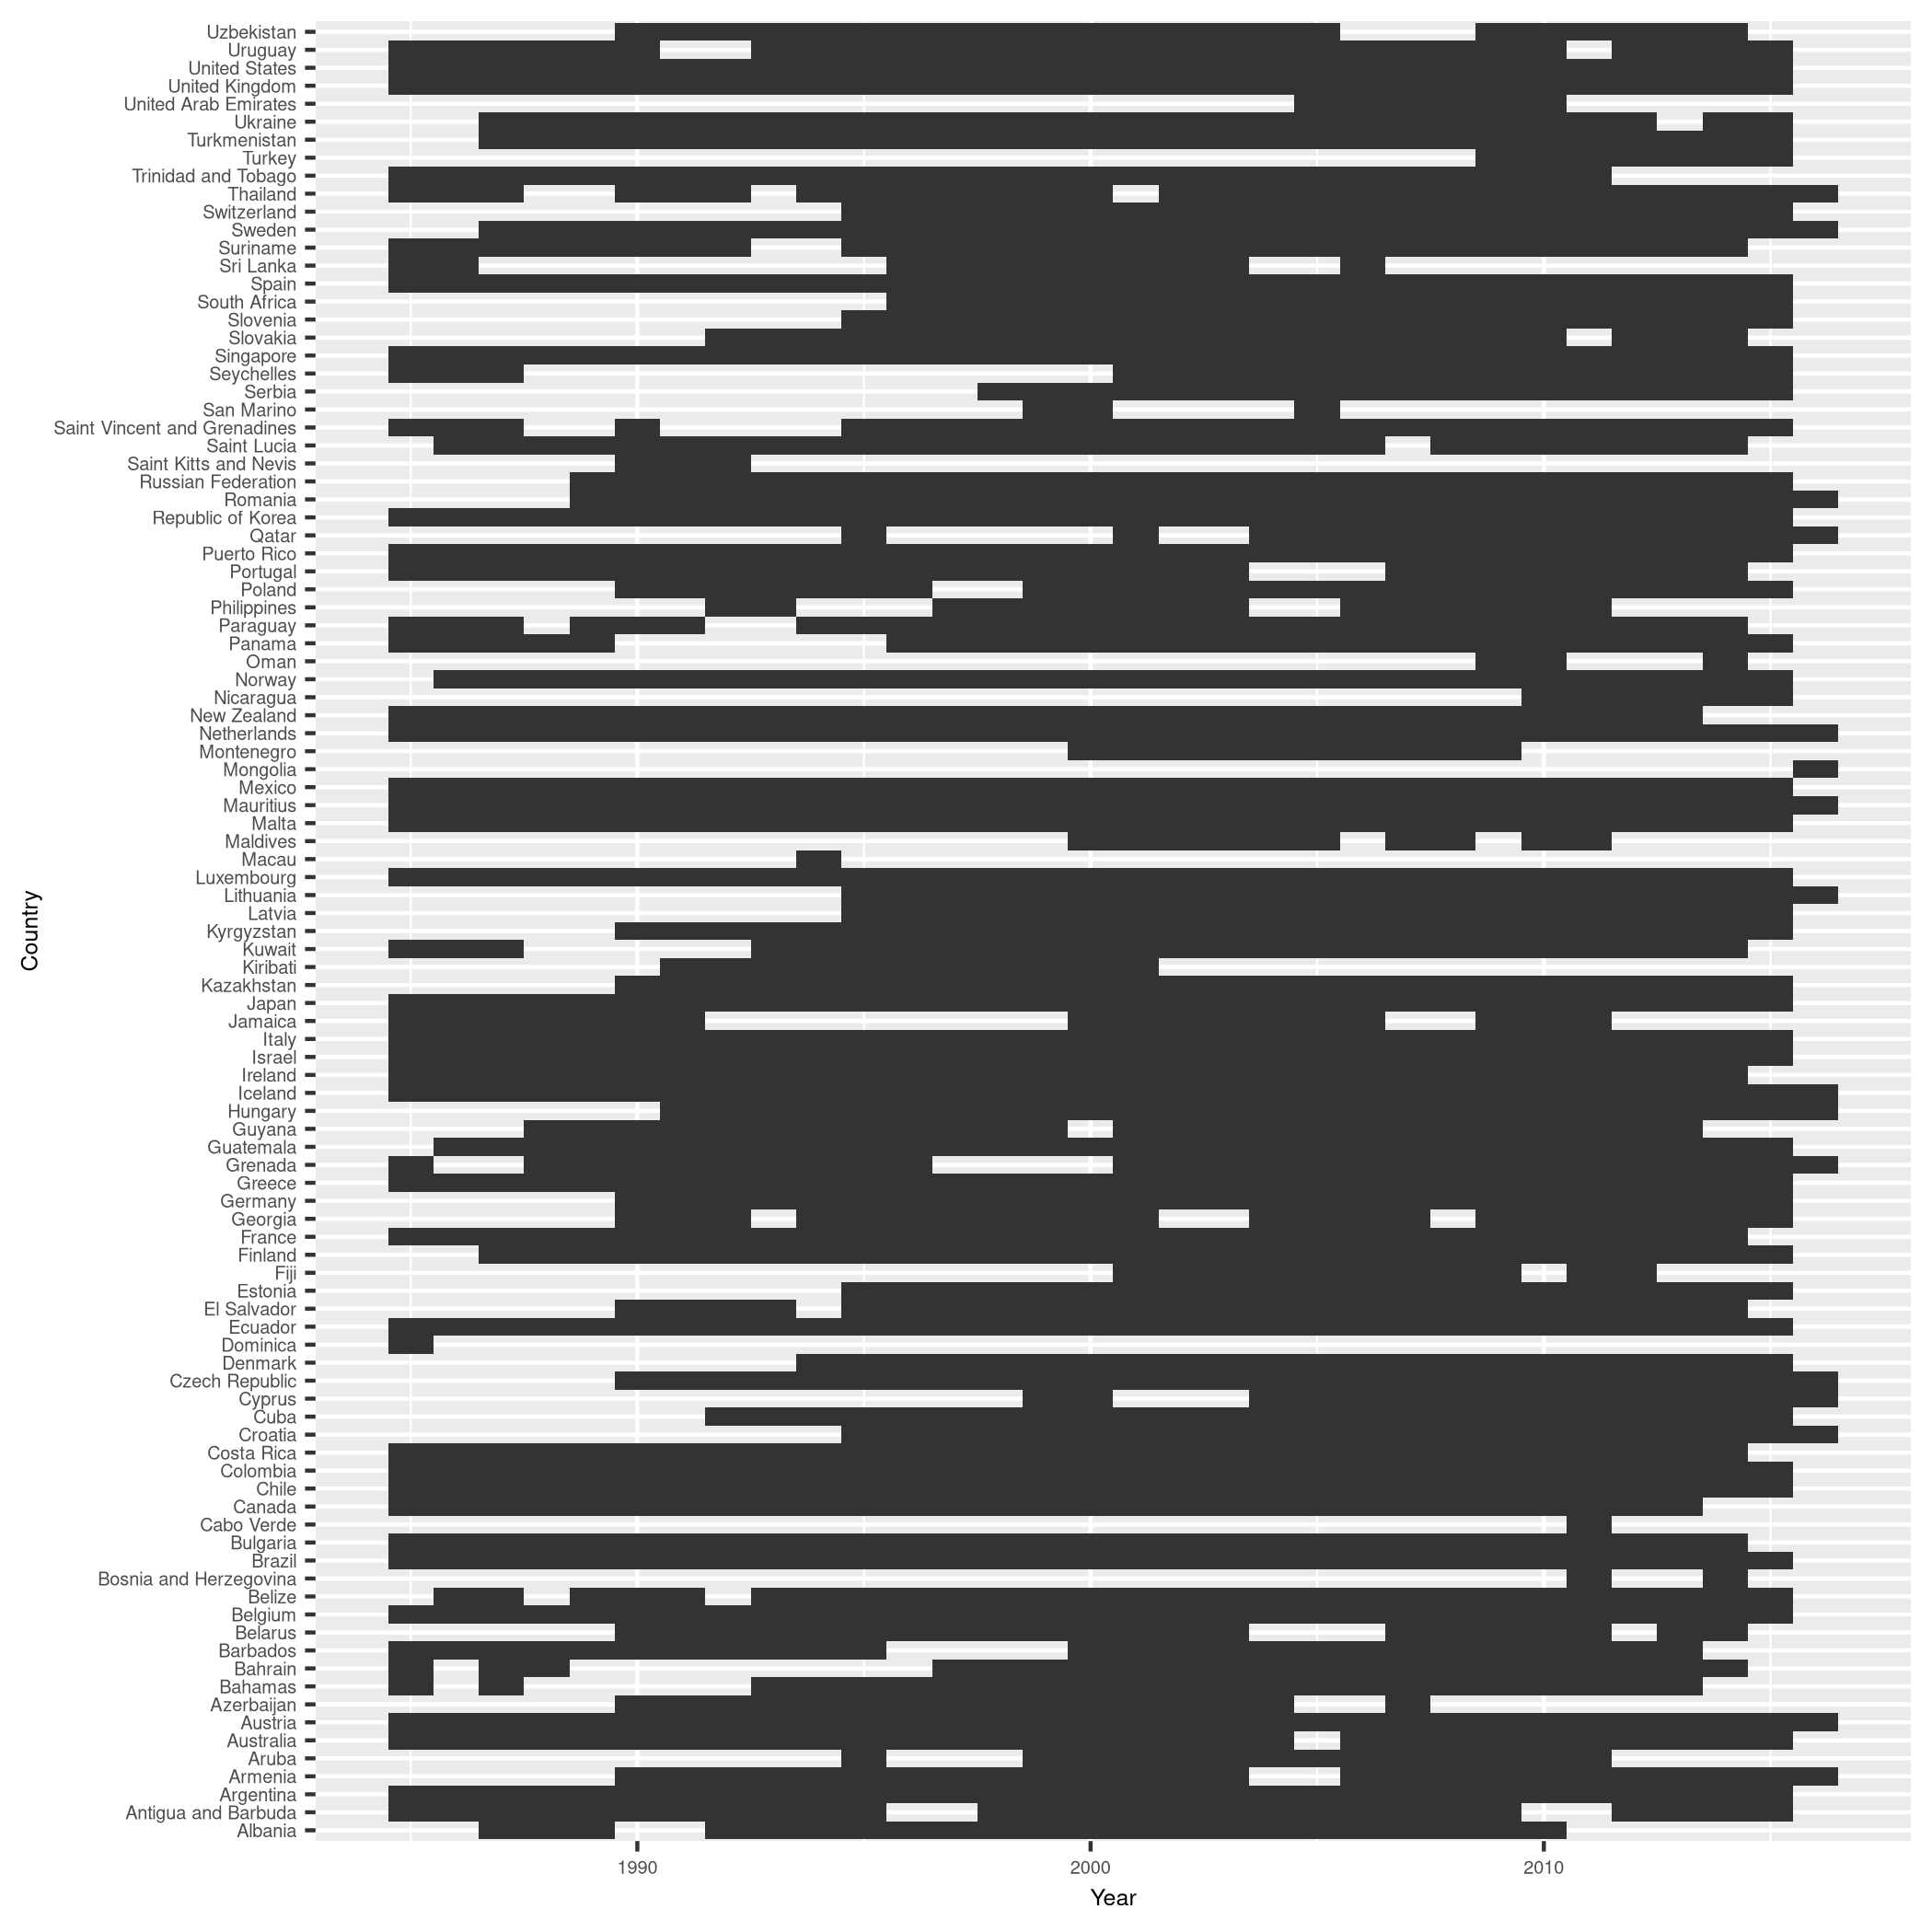
\includegraphics[width=1.25\textwidth]{1-available-data.png}}
    \caption{Available data per Country and Year}
    \label{fig:available-data}
\end{figure}

Figure \imgref{fig:available-data} shows the data set is all but complete. The dark tiles show years for which data of a country is available, light tiles represent missing data. Some countries have very few data points, whereas others have data for most of the years. The less yearly data is available, the harder an assessment of the development for a single country becomes.

\begin{figure}
    \centering
    \makebox[\textwidth][c]{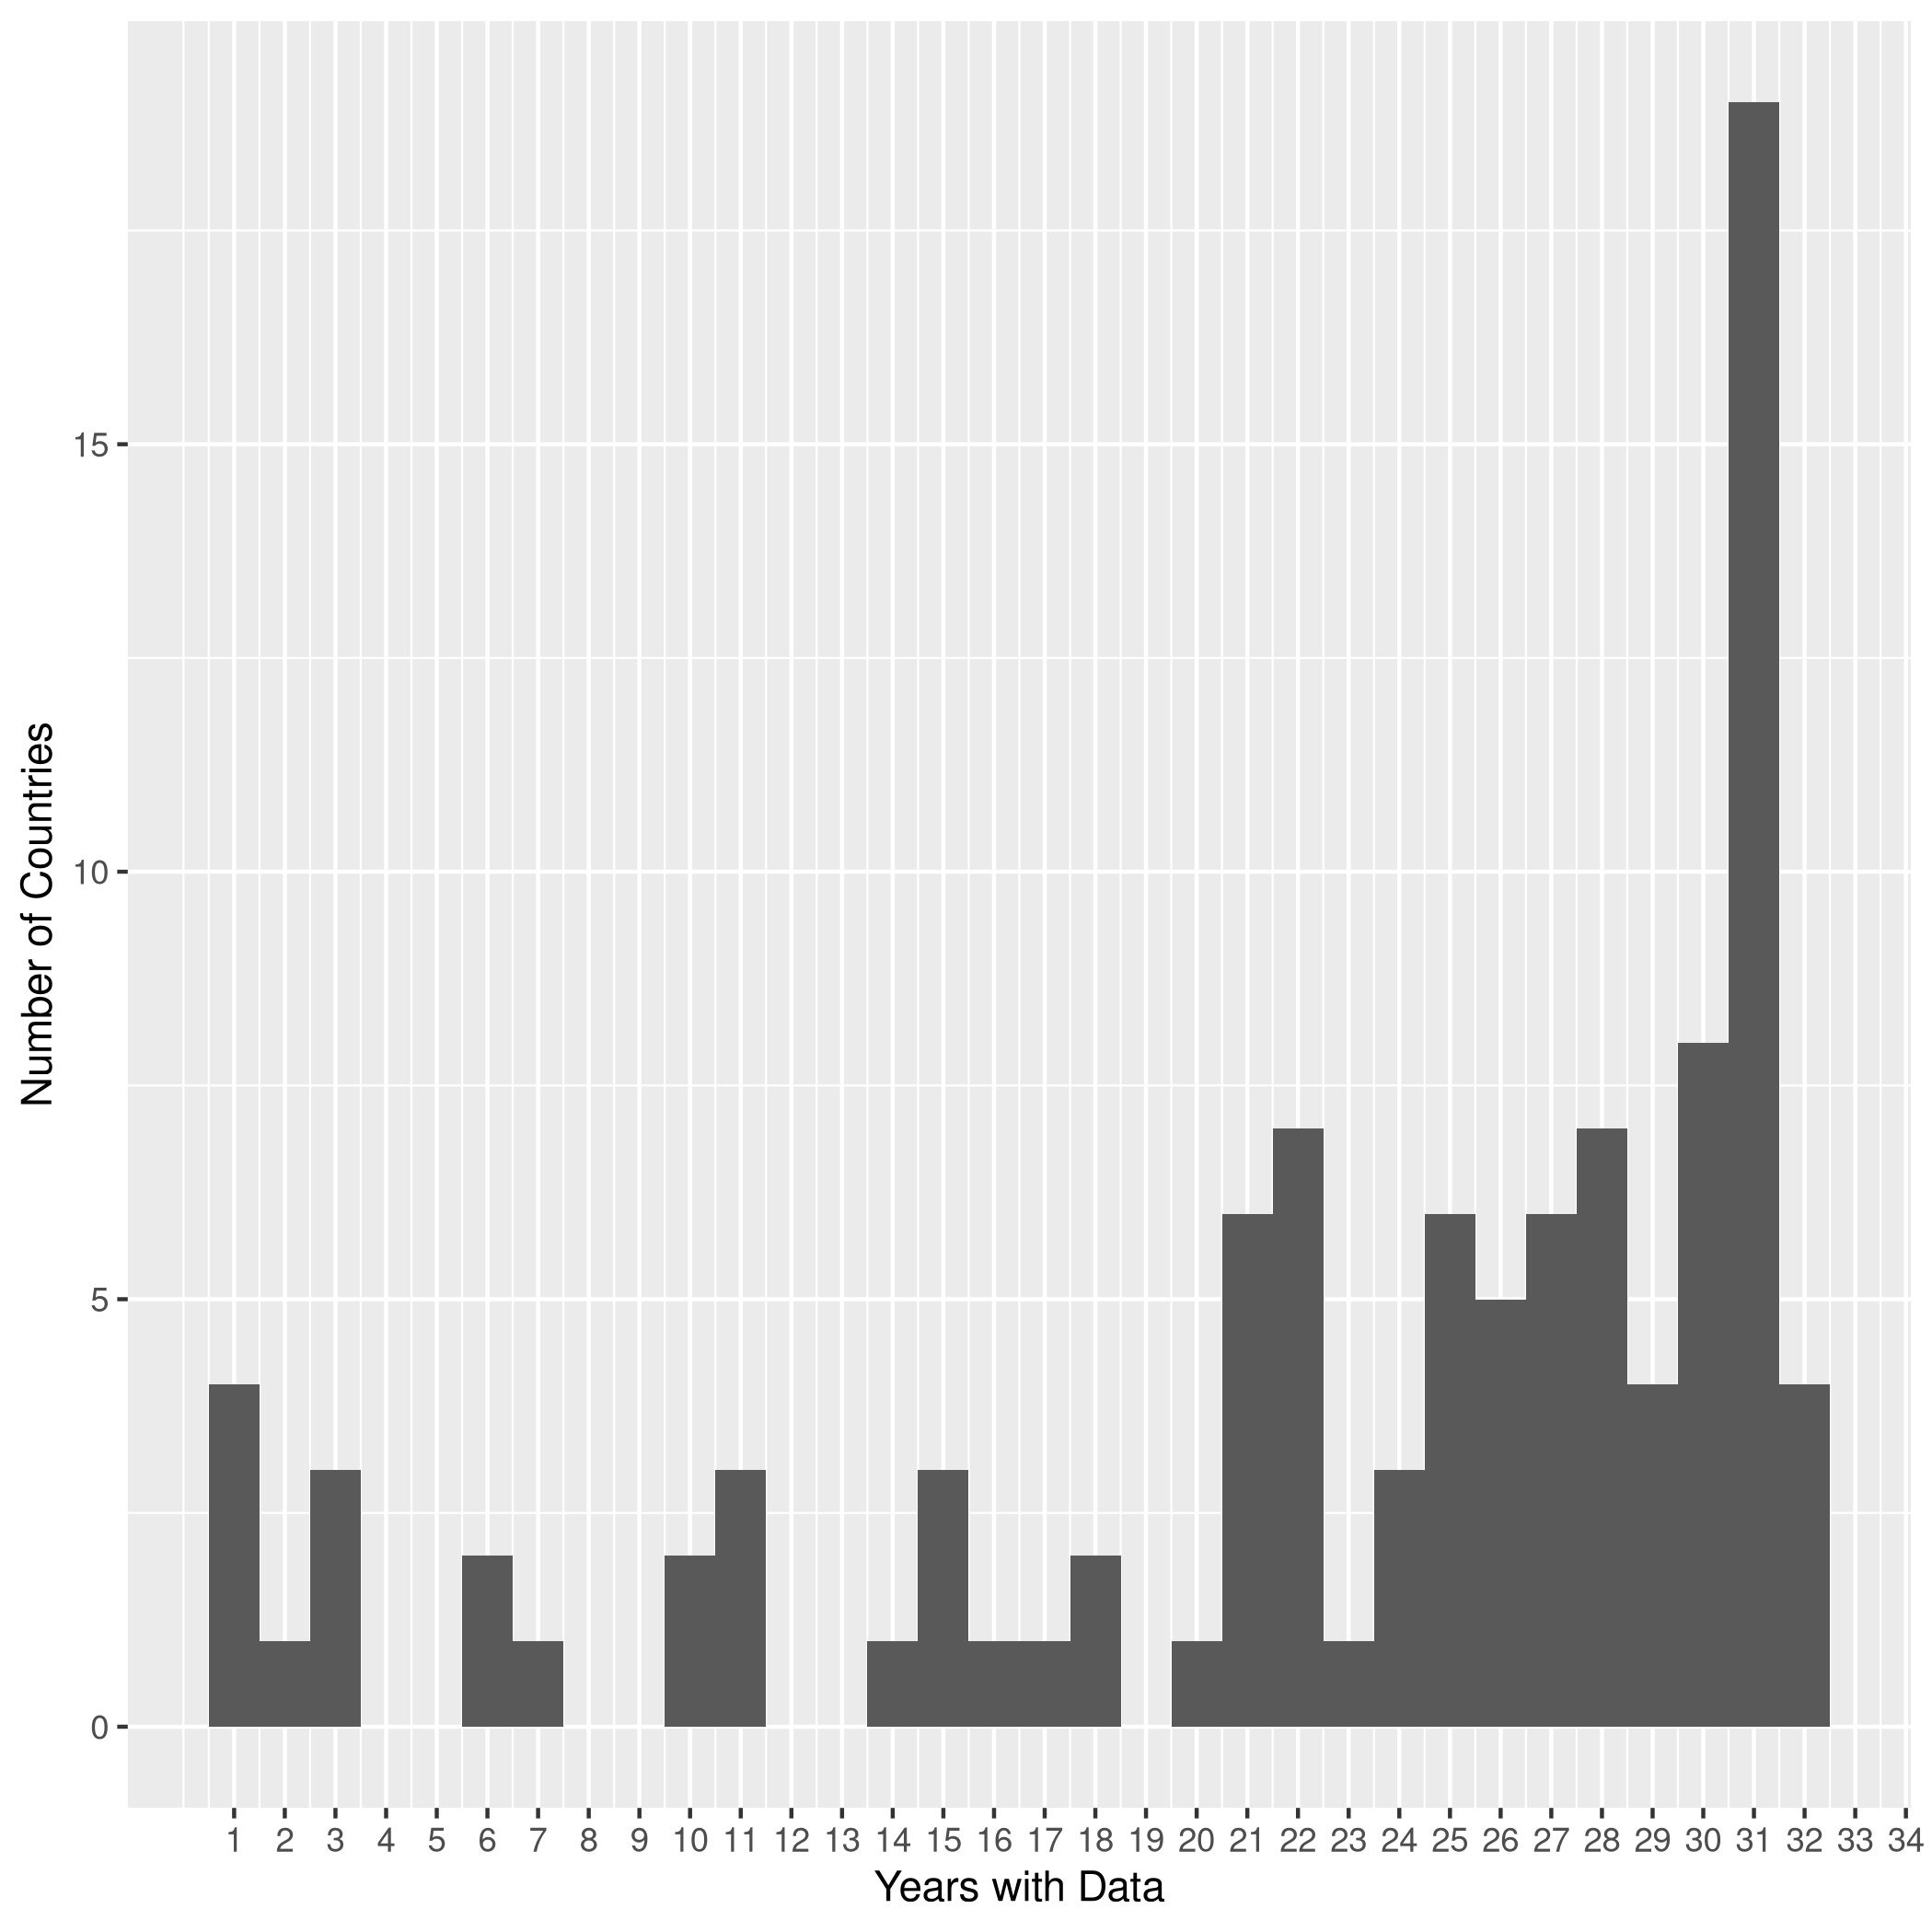
\includegraphics[width=1.25\textwidth]{2-observations-histogram.png}}
    \caption{Histogram Showing the Number of Measurements per Country}
    \label{fig:observations-histogram}
\end{figure}

The same data is summarized in figure \imgref{fig:observations-histogram}, which quantifies the number of observations that are available per country.

\begin{figure}
    \centering
    \makebox[\textwidth][c]{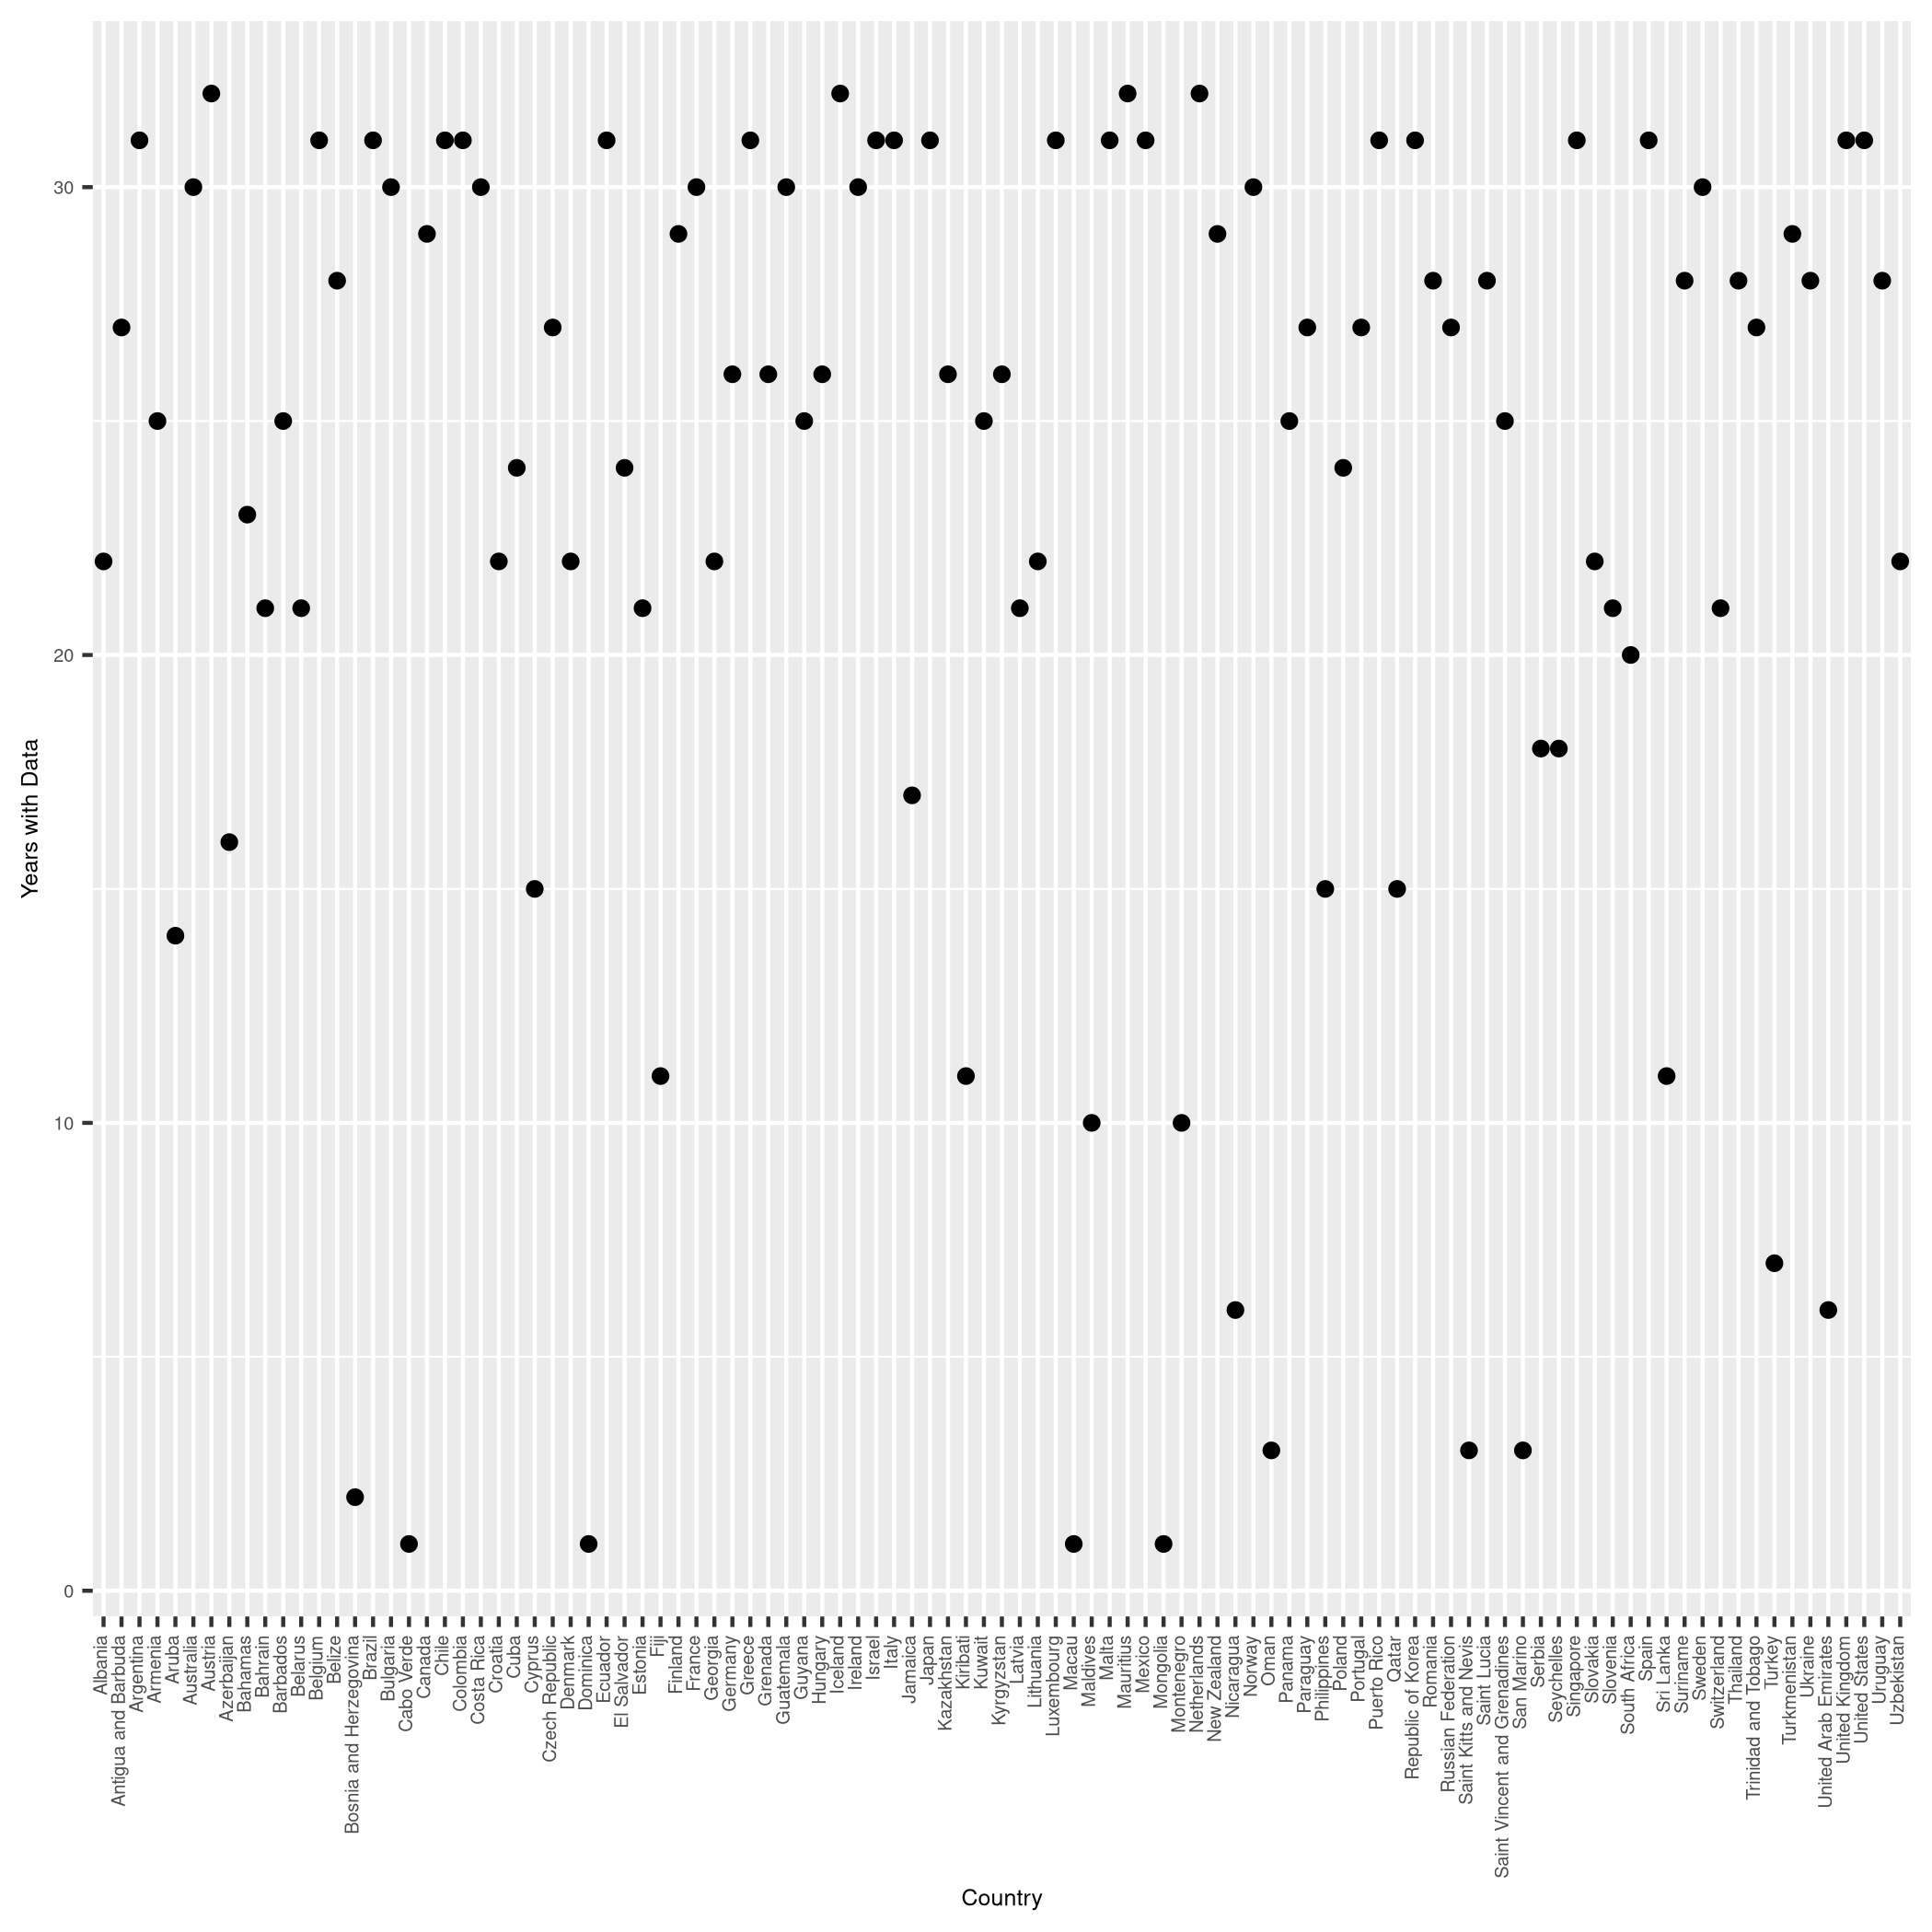
\includegraphics[width=1.25\textwidth]{3-years-with-data.png}}
    \caption{Numbers of Years with Suicide Data Provided per Country}
    \label{fig:years-with-data}
\end{figure}

Figure \imgref{fig:years-with-data} provides summarized insight into invidivual countries.
